%!TEX root=kdd15_workshop_main.tex
\section{Evaluation}

We ran our distributed experiments on the Edison machine at NERSC, featuring 5576 compute nodes with two 12-core Intel ``Ivy Bridge'' processors per node, and a Cray Aries interconnect. For scalability experiments we generated undirected Kronecker graphs of varying scale in parallel using the Graph500 Reference implementation~\cite{graph500}. 

We also measured the overall quality of partitions by the \textit{fraction of cut edges} $\lambda$.
\begin{align}\lambda = \frac{\text{Number of edges cut by partition}}{\text{Total number of edges}}\end{align}
The fraction of edges cut demonstrates the quality of the edge minimization aspect of partitioning the graph.

As a baseline, we can compare this to the expected quality of a random $k-$partition:
\begin{align}\lambda_r = \frac{k^2 - k}{k^2} = \frac{k-1}{k} \end{align}

Any partitioner that produces partitions with $\lambda < \lambda_r$ has improved the parallel locality of the partitions. 
We present $\lambda_{r,k}$ along with our one-pass, real network results in Table \ref{table:big}.

\subsection{Test Graphs}
We tested \ourmethod on both real and synthetic networks.
Real networks demonstrate \ourmethod's potential for use on real domain problems.
We also utilized synthetic graphs, because they allow better experimental control over size and structure.
\subsubsection{Real-world Graphs}
The SNAP dataset is a collection of real-world networks collected by Leskovec and collaborators~\cite{Leskovec-data, snapnets}. 
Many networks in the collection are power-law and scale-free representatives of social networks (such as collaboration networks, citation networks, email networks, and web graphs). We consider these to be ideal targets for streaming partitioning, because these domains are producing the vast majority of the `big-data' that is difficult to partition using traditional methods.

% We also speculate (but have no proof) that the `random' structure of scale-free networks better suits the random quality of streaming graph partitioning, whereas a spatially-oriented graph would be poorly suited (for instance, in a grid, a streaming partitioner would create many local pockets for one particular partition, whereas a spatial partitioner would recognize that the graph could be geometrically bisected).

\subsection{Quality}
In Table~\ref{table:big} we show some properties of our real test-graphs, as well as the performance of our streaming partitioner on them, for $k=2$ and $k=8$.
% As a note, the ratio of change in $\lambda$ from $k=2$ to $k=8$ was for the vast majority of cases within 1.5 and 2.2. 
% This suggests good scalability.


\begin{figure*}
\caption{Basic properties of graphs in SNAP data set~\cite{Leskovec-data}, and $\lambda$ for one pass. $\lambda_{r,2}=0.5,\lambda_{r,8}=0.87$}
\rowcolors{2}{blue!05}{blue!15}
\centering
{ \begin{tabular}{ *7l }    \toprule
\label{table:big}
\emph{Data Set} & $N$ & $nnz$ & \emph{sym} & \emph{power-law?} & $\lambda, k=2$ & $\lambda, k=8$ \\\midrule
amazon0302 & 262111 & 1234877 & no & yes & 0.202&0.37\\
% amazon0312 & 400727 & 3200440 & no & yes & 0.212&0.38\\
% amazon0505 & 410236 & 3356824 & no & yes & 0.206&0.37\\
% amazon0601 & 403394 & 3387388 & no & yes & 0.203&0.36\\
% as-735 & 7716 & 26467 & yes & yes & 0.207&0.44\\
as-Skitter & 1696415 & 22190596 & yes & yes & 0.166&0.324\\
ca-AstroPh & 18772 & 396160 & yes & yes & 0.232&0.413\\
% ca-CondMat & 23133 & 186936 & yes & yes & 0.214&0.398\\
% ca-GrQc & 5242 & 28980 & yes & yes & 0.128&0.241\\
% ca-HepPh & 12008 & 237010 & yes & yes & 0.082&0.192\\
% ca-HepTh & 9877 & 51971 & yes & yes & 0.202&0.378\\
cit-HepPh & 34546 & 421578 & no & yes & 0.343&0.646\\
% cit-HepTh & 27770 & 352807 & no & yes & 0.360&0.605\\
cit-Patents & 3774768 & 16518948 & no & yes & 0.402&0.726\\
% email-Enron & 36692 & 367662 & yes & yes & 0.132&0.407\\
email-EuAll & 265214 & 420045 & no & yes & 0.280&0.538\\
Oregon-1 & 11492 & 46818 & yes & yes & 0.224&0.406\\
% Oregon-2 & 11806 & 65460 & no & yes & 0.185&0.429\\
p2p-Gnutella04 & 10879 & 39994 & no & yes & 0.415&0.747\\
roadNet-CA & 1971281 & 5533214 & yes & no & 0.186&0.36\\
% roadNet-PA & 1090920 & 3083796 & yes & no & 0.188&0.36\\
% roadNet-TX & 1393383 & 3843320 & yes & no & 0.185&0.358\\
% soc-Epinions1 & 75888 & 508837 & no & yes & 0.173&0.34\\
soc-LiveJournal1 & 4847571 & 68993773 & no & yes &0.234& 0.463\\
% soc-sign-epinions & 131828 & 841372 & no & yes &0.173&0.34\\
% soc-Slashdot0811 & 77360 & 905468 & no & yes &0.179&0.417\\
soc-Slashdot0902 & 82168 & 948464 & no & yes &0.236&0.382\\
% web-BerkStan & 685230 & 7600595 & no & yes &0.187&0.301\\
web-Google & 916428 & 5105039 & no & yes &0.189&0.336\\
% web-NotreDame & 325729 & 1497134 & no & yes &0.204&0.345\\
% web-Stanford & 281903 & 2312497 & no & yes &0.154&0.34\\
wiki-Talk & 2394385 & 5021410 & no & yes &0.411&0.752\\
% wiki-Vote  & 8297 & 103689 & no & yes &0.409&0.688\\
 \hline
\end{tabular}\par
}
\end{figure*}



% We also note Figure~\ref{fig:4}, which illustrates the result of the streaming algorithm on a more spacial network (roadNet-CA). The `local' nonzeros are those points in the 8 diagonal blocks, while the `remote' edges are those outside. While a good partitioner would concentrate the vast majority of elements along the diagonal (which is possible because the graph has very high diameter), the streaming partitioner fails to recognize this quality, and each partition has vertices distributed somewhat randomly through the network. Nonetheless, the partition is decent (only 18 percent of edges are cut).

% \begin{figure}[h!]
% \centering
% 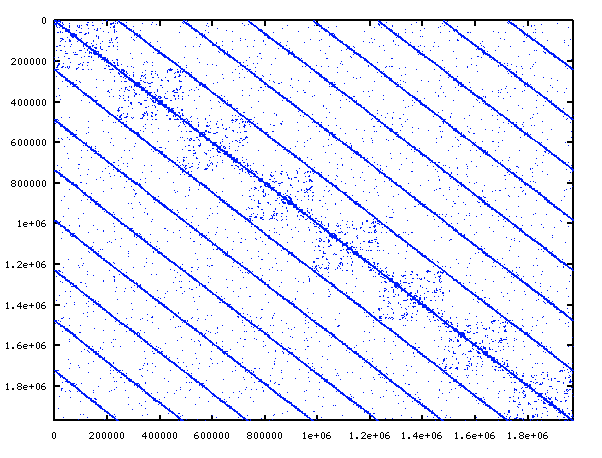
\includegraphics[width=0.8\columnwidth] {figures/roadNet-CA8.png}
% \caption[Caption for]{Spy plot of roadNet-CA 8-partition ($\lambda=0.177$). This illustrates how a streaming algorithm cannot take into account the spatial/planar properties of a graph.}
% \label{fig:4}
% \end{figure}

\subsubsection{Synthetic Graphs}
To generate the test graphs we used the Graph500 Kronecker-Graph generator.
Kronecker graphs are commonly used in HPC graph benchmarks and testing and can be scaled arbitrarily large for testing purposes. 


% In Figure~\ref{fig:kronspeed} however, we increase the $p$-value on a single ER graph. We see that the partition quality significantly decreases. 
% This is to be expected of all partitioners in general. In fact, for E-R graphs, the critical $p$-value for which the optimal edge cut is equal to the expected average random partition is relatively simple to identify~\cite{journals/cj/GanleyH94}

\paragraph{Restreaming \& Additional Passes}
A key facet of \ourmethod is performing additional passes of partitioning on a pre-partitioned graph. 
The partitioner is fast enough that it is faster to do $n$ streaming passes than use a slower mainstream graph partitioner.
To explore this idea, we perform a number of passes on the SNAP data set, and observe the effects of various graphs (see Figure~\ref{fig:01, fig:02}). 

The algorithm is simple: once we have computed the first partition, we retain the original partition mapping. 
Then, as we make another pass, we compute the new objective function using the partition mapping that has already been filled in. 
Vertices may be switched to new partitions. 
This mitigates poor partitioning decisions that sometimes occur at the beginning of the algorithm, when there was not as much information.

Figures~\ref{fig:01} and \ref{fig:02} show the improvement of $\lambda$ as we continue to make passes over selected networks. 
The second pass usually exhibits the best improvement, while subsequent passes offer diminishing returns.
Making a low-cut 16-partitioning is considerably harder than the 2-partition case, explaining the difference in quality in Figure~\ref{fig:02}.


% We hope to contrast this performance to that of METIS in the future. (We have implemented a METIS partitioner for comparison but it currently encounters a segmentation faults with some frequency).



\begin{figure}[h!]
\centering
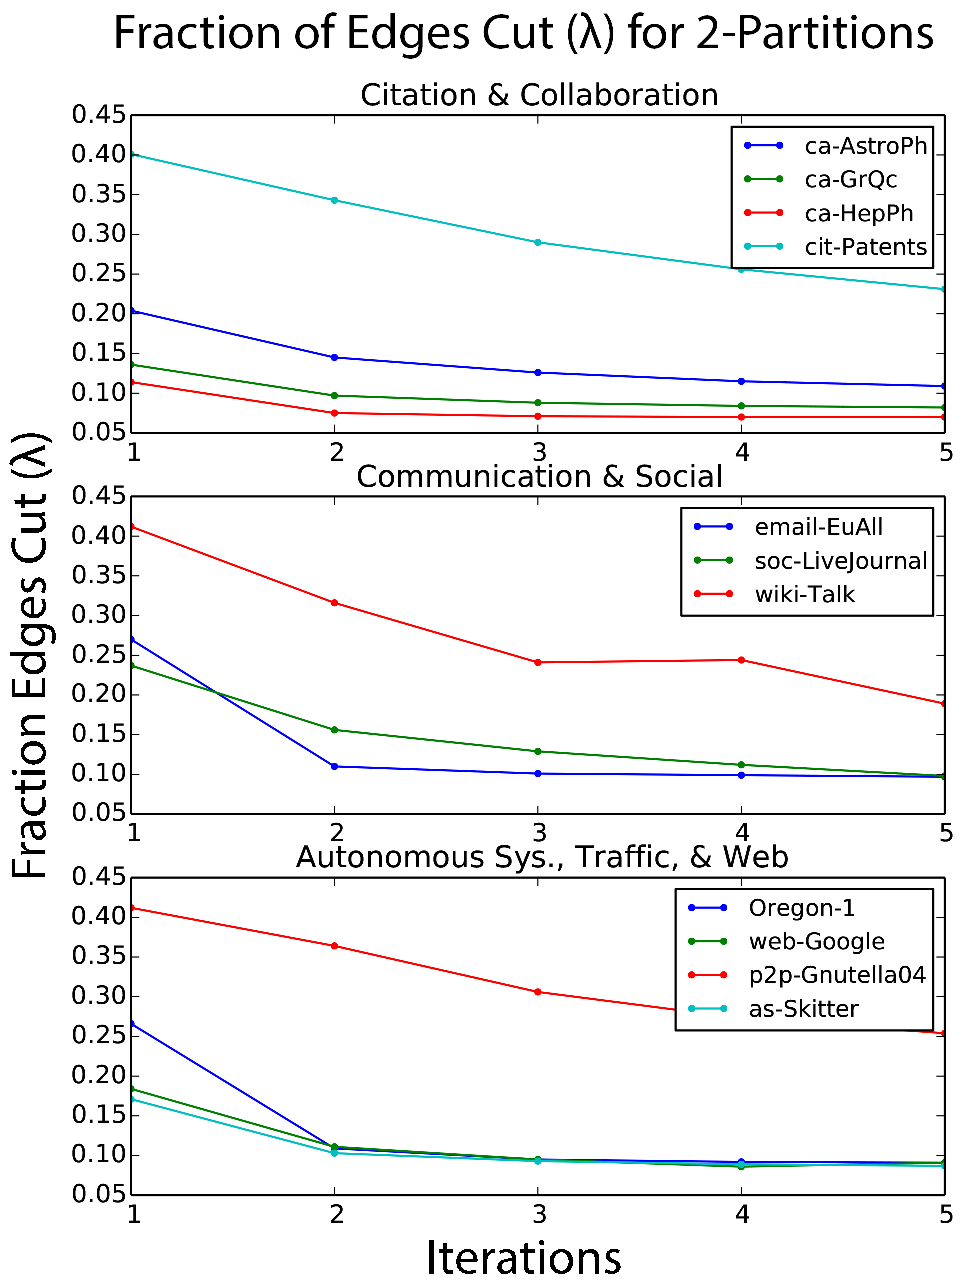
\includegraphics[width=0.9\columnwidth] {figures/real_k2_lambda.pdf}
\caption[Caption for]{Improvement in the edges cut ($\lambda$) over 5 passes for bi-partitions of each graph. Because there are only two partitions, the algorithm is able to quickly fix mistakes it made in the initial partitioning. Many of the errors made in the first pass are fixed in the second iteration, with diminishing improvement thereafter.}
\label{fig:01}
\end{figure}

\begin{figure}[h!]
\centering
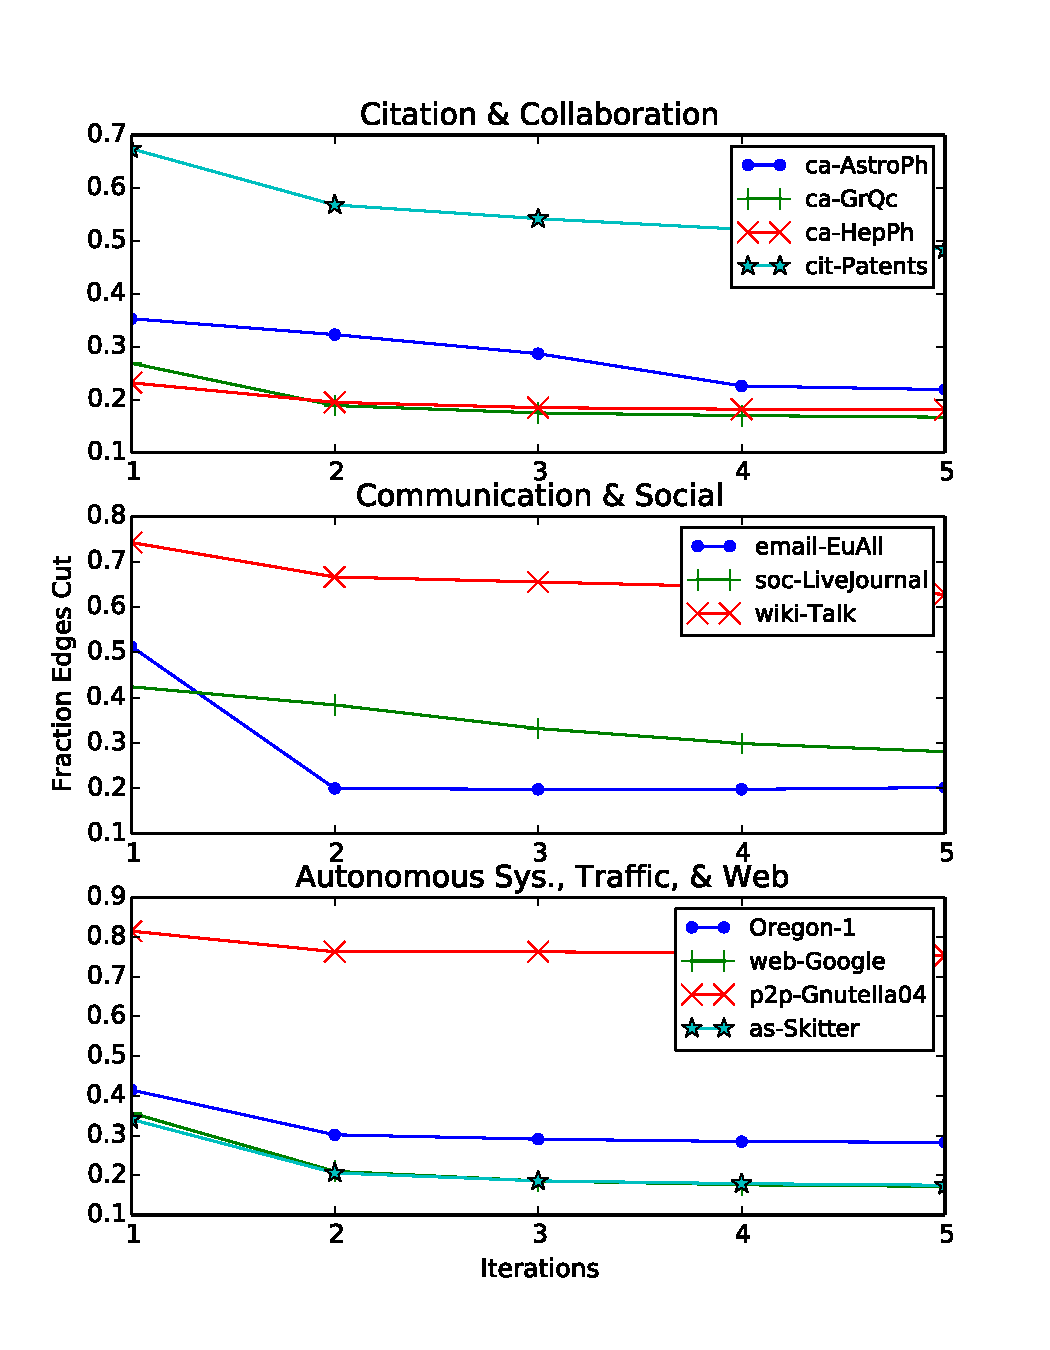
\includegraphics[width=0.9\columnwidth] {figures/real_k16_lambda.pdf}
\caption[Caption for]{Improvement in edges cut ($\lambda$) over 5 passes for $k=16$-partitions of each graph. Dividing the graph into 16 partitions makes the minimum edge cut problem much more challenging. Similar to the bi-partition results, we experience the best gain in the second pass and less in subsequent passes.}
\label{fig:02}
\end{figure}

% \begin{figure}[h!]
% \centering
% 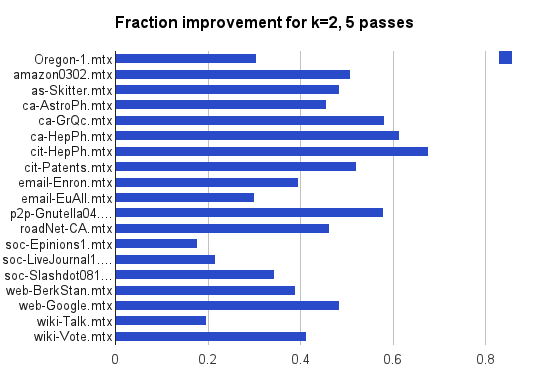
\includegraphics[width=0.8\columnwidth] {figures/2partfrac}
% \caption[Caption for]{Improvement in $\lambda_{initial}/\lambda_{5}$ after running 5 passes for bi-partitions of each graph. After 5 passes all partitions had significantly improved in edge-cut quality.}
% \label{fig:03}
% \end{figure}

% \begin{figure}[h!]
% \centering
% 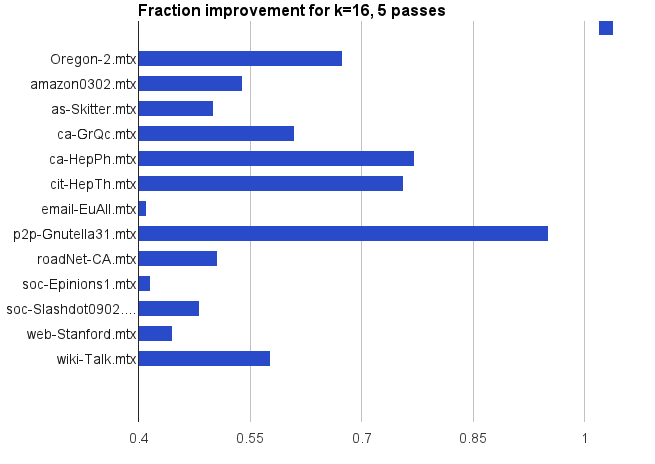
\includegraphics[width=0.8\columnwidth] {figures/16partfrac}
% \caption[Caption for]{Improvement in $\lambda_{initial}/\lambda_{5}$ after running 5 passes for 16-partitions of each graph.}
% \label{fig:04}
% \end{figure}

\begin{figure}[h!]
\centering
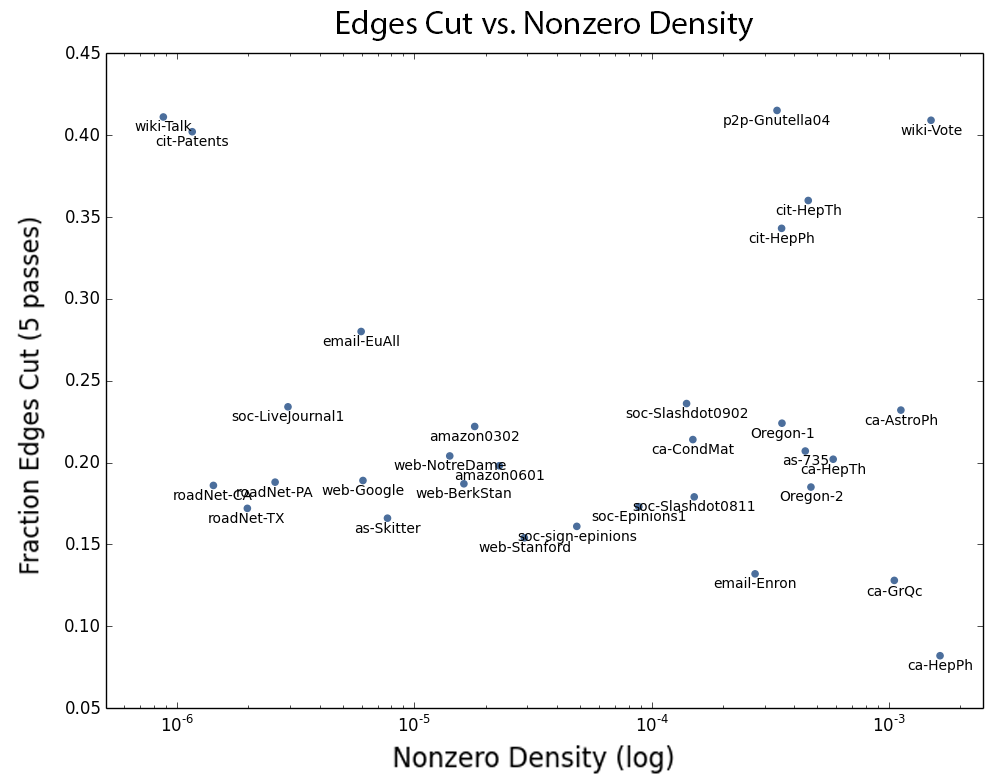
\includegraphics[width=0.98\columnwidth] {figures/cutvsdensity}
\caption[Caption for]{Cut quality vs nonzero density for the real SNAP networks. The graph shows little noticeable correlation.}
\end{figure}

\subsection{Scalability}
In order to test the scalability of \ourmethod we used a series of Kronecker graphs running on a state-of-the-art system.
In Figure~\ref{fig:kronqual} we illustrate the streaming graph partitioner on Kronecker graphs with a widely varying number of nodes.
We show the Kronecker graphs performance in Figure!\ref{fig:kronspeed}. 
\ourmethod is able to achieve a good balance between quality at incredible speeds.


\begin{figure}[h!]
\centering
  
\includegraphics[width=0.8\columnwidth]{figures/kronecker_quality_tests.pdf}
  \caption{Partition quality of various Kronecker graphs.}
  \label{fig:kronqual}
\end{figure}

\begin{figure}[h!]
\centering
  
\includegraphics[width=0.8\columnwidth]{figures/kronecker_speed_tests.pdf}
  \caption{Partition speed of various Kronecker graphs.}
  \label{fig:kronspeed}
\end{figure}


\subsection{Analysis}
% Other data from real-world was harder to analyze -- there are not enough wide differences between data sets' results to draw strong conclusions.
Despite the complexity of many of the real graphs, \ourmethod creates well-balanced partitions.
While Power-Law graphs are overwhelmingly considered to be difficult to partition~\cite{Abou-Rjeili:2006:MAP:1898953.1899055}, we have demonstrated that a very simple, fast, algorithm is capable of significantly reducing communication in their parallel computation. 
We also demonstrate in Figures~\ref{fig:1, fig:2} that additional passes can further reduce edges cut (by up to a factor of 3). 

% Isolated comparisons we have made to the state-of-the-art partitioner METIS show that these results are competitive (usually within a factor of 2).
In Figure~\ref{fig:metis}, \ourmethod performs comparably with parMETIS.  
Streaming partitioning is a valid alternative to conventional offline approaches and can be integrated in distributed-memory, on-the-fly algorithms for big-data.

One set of outlying (poorly-performing) data points are the Gnutella networks.
While Gnutella networks exhibit power-law-like topologies, elements of their algorithm truncate nodes from ever becoming extremely large. 
This heavy-clipping sets the Gnutella networks apart from many of the other social network topologies in our experiments.
The data set also has extremely low clustering coefficients and a very small number of closed triangles \cite{Ripeanu:2002:MGN:613352.613670}. 
Low clustering coefficients decrease the chance that neighbors of the current node-under-consideration share a partition. 
With more neighbors distributed across the partitions, many partitions will have roughly the same score, making optimal partition choices much harder.

A danger of naively running multiple passes is that one partition often becomes populated by very high-degree vertices. 
We attribute this to the ``dense core'' surrounded by a less-dense periphery that many scale-free graphs possess.
This can be observed qualitatively when scale-free graphs are embedded in a spectral space~\cite{Lang04findinggood}.

This dense partition tends to strongly emerge as we continue to make further passes of the streaming algorithm.
In order to overcome this we used the tempered parameter technique described in our methodology section. 

\begin{figure}[h!]
\centering
  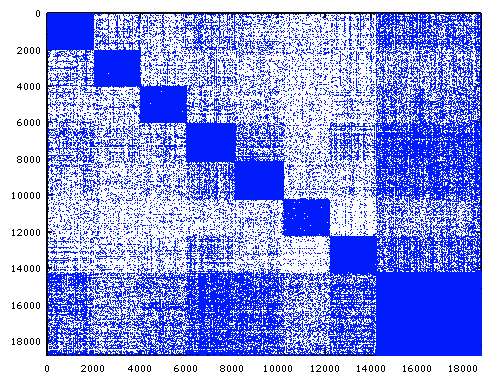
\includegraphics[width=0.8\columnwidth]{figures/astroPh8.png}
  \caption{Spy plot of ca-AstroPh 8-partition ($\lambda=0.253$). Note the denser, high-degree subgraph.}
  \label{fig:dense}
\end{figure}


